% ============================================================
% Musical Intelligence — Progress Update for Prof. David Poeppel
% March 2026
% ============================================================
\documentclass[11pt]{article}

\usepackage[utf8]{inputenc}
\usepackage[T1]{fontenc}
\usepackage{mathpazo}
\usepackage[margin=2.2cm]{geometry}
\usepackage{graphicx}
\usepackage{booktabs}
\usepackage{amsmath,amssymb}
\usepackage{xcolor}
\usepackage{hyperref}
\usepackage{natbib}
\usepackage{caption}
\usepackage{subcaption}
\usepackage{enumitem}
\usepackage{tikz}
\usepackage{tabularx}
\usepackage{float}
\usepackage{microtype}
\usepackage{fancyhdr}
\usepackage{siunitx}

\usetikzlibrary{arrows.meta,positioning,shapes.geometric,fit}

\definecolor{miblue}{HTML}{2171B5}
\definecolor{migreen}{HTML}{238B45}
\definecolor{mired}{HTML}{CB181D}
\definecolor{migray}{HTML}{636363}

\hypersetup{colorlinks=true, linkcolor=miblue, citecolor=migreen, urlcolor=miblue}
\captionsetup{font=small, labelfont=bf, labelsep=period}

\pagestyle{fancy}
\fancyhf{}
\renewcommand{\headrulewidth}{0.3pt}
\fancyhead[L]{\small\itshape Musical Intelligence — Progress Update}
\fancyhead[R]{\small\thepage}

\graphicspath{{../figures/}}

\newcommand{\rthree}{R\textsuperscript{3}}
\newcommand{\hthree}{H\textsuperscript{3}}
\newcommand{\cthree}{C\textsuperscript{3}}

% ============================================================
\begin{document}

\begin{center}
{\Large\bfseries Musical Intelligence:\\[3pt]
A Computational Architecture for Music Cognition}\\[10pt]
{\large Progress Update — March 2026}\\[6pt]
{\normalsize Ama\c{c} Erdem}\\[2pt]
{\small\itshape ali@srcmusicalintelligence.com}\\[12pt]
\rule{0.7\textwidth}{0.4pt}
\end{center}

\vspace{6pt}

\noindent Dear Prof.\ Poeppel,

\smallskip
\noindent Thank you again for your thoughtful feedback last August. I took both suggestions seriously. First, regarding brain localization: I completely rebuilt the Region Activation Map using literature-sourced MNI152 coordinates with per-region citations (detailed in Section~\ref{sec:localization}). Second, regarding focus: rather than trying to solve everything, I narrowed the six-month effort to \emph{one question}:

\begin{quote}
\itshape Can a single deterministic architecture, processing only raw audio, generate predictions that align with empirical data across multiple domains of music cognition?
\end{quote}

\noindent The answer, across seven validation studies and 34 automated tests, is a qualified yes --- strong in some domains, preliminary in others. Below is a concise summary of the architecture and results.

% ============================================================
\section{Architecture Overview}
% ============================================================

Musical Intelligence (MI) is a three-layer computational pipeline implemented in 756 Python modules. It takes raw audio as input and produces three output streams: 26 brain-region activation estimates, 4 neurochemical channels, and 6 experiential domains.

\begin{figure}[h]
\centering
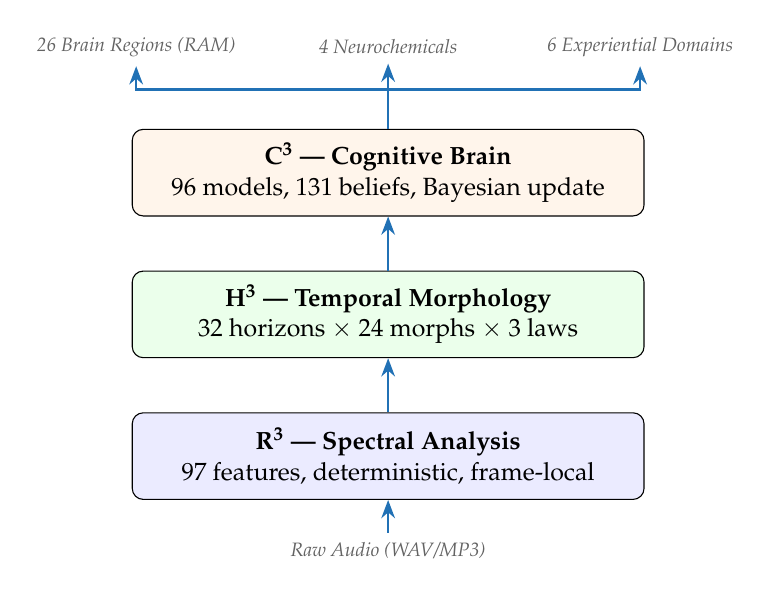
\begin{tikzpicture}[
    >=Stealth,
    layer/.style={draw, rounded corners=4pt, minimum width=6.5cm, minimum height=1.1cm, font=\small, align=center},
    arrow/.style={->, thick, miblue},
    note/.style={font=\scriptsize\itshape, text=migray},
]
% Layers
\node[layer, fill=blue!8] (r3) at (0,0) {\textbf{\rthree{} — Spectral Analysis} \\ 97 features, deterministic, frame-local};
\node[layer, fill=green!8] (h3) at (0,1.8) {\textbf{\hthree{} — Temporal Morphology} \\ 32 horizons $\times$ 24 morphs $\times$ 3 laws};
\node[layer, fill=orange!8] (c3) at (0,3.6) {\textbf{\cthree{} — Cognitive Brain} \\ 96 models, 131 beliefs, Bayesian update};

% Input/Output
\node[note] (audio) at (0,-1.2) {Raw Audio (WAV/MP3)};
\node[note] (ram) at (-3.2, 5.2) {26 Brain Regions (RAM)};
\node[note] (neuro) at (0, 5.2) {4 Neurochemicals};
\node[note] (psi) at (3.2, 5.2) {6 Experiential Domains};

% Arrows
\draw[arrow] (audio) -- (r3);
\draw[arrow] (r3) -- (h3);
\draw[arrow] (h3) -- (c3);
\draw[arrow] (c3.north) -- ++(0, 0.5) -| (ram.south);
\draw[arrow] (c3.north) -- (neuro.south);
\draw[arrow] (c3.north) -- ++(0, 0.5) -| (psi.south);
\end{tikzpicture}
\caption{MI processes raw audio through three layers. \rthree{} extracts 97 spectral features per frame. \hthree{} computes multi-scale temporal statistics (8,600 active tuples from a 223k theoretical space). \cthree{} runs 96 biologically-grounded models that update 131 probabilistic beliefs via precision-weighted Bayesian inference.}
\label{fig:arch}
\end{figure}

\paragraph{Key design principles.}
\begin{itemize}[nosep,leftmargin=1.5em]
    \item \textbf{Raw audio in, structured cognition out.} No symbolic input (MIDI, scores). Everything is derived from the waveform.
    \item \textbf{Deterministic and interpretable.} Same audio $\rightarrow$ same output. Every belief traces to specific mechanisms with literature citations.
    \item \textbf{Frozen interfaces.} \rthree{} and \hthree{} are version-locked (v1.0.0). Only \cthree{} models evolve.
    \item \textbf{Evidence-tiered.} Each of the 96 mechanism models carries an explicit evidence tier ($\alpha$: mechanistic, $\beta$: integrative, $\gamma$: speculative) with falsification criteria.
\end{itemize}

% ============================================================
\section{Addressing Brain Localization}
\label{sec:localization}
% ============================================================

You correctly identified that the previous localization was problematic. The midline activations were an artifact of how coordinates were projected onto the visualization surface.

I rebuilt the Region Activation Map (RAM) from scratch:

\begin{itemize}[nosep,leftmargin=1.5em]
    \item \textbf{26 regions} across three groups: 12 cortical (with Brodmann areas), 9 subcortical, 5 brainstem.
    \item \textbf{Literature-sourced MNI152 coordinates.} Every region's centroid is taken from published atlases and meta-analyses (e.g., A1/HG at [48, $-$18, 8] from \citealt{morosan2001}; NAcc at [10, 12, $-$6] from \citealt{knutson2005}).
    \item \textbf{594 total citations} across all 26 regions (mean 16.5 per cortical region).
    \item \textbf{Activation is accumulative, not localized \emph{de novo}.} Each region receives weighted contributions from specific \cthree{} mechanism outputs (44 relay-to-region links). The weights represent coupling strengths from literature, not learned parameters.
\end{itemize}

\noindent To be clear about what RAM is and is not:

\begin{itemize}[nosep,leftmargin=1.5em]
    \item RAM is \textbf{not} a neural imaging prediction. It is a \emph{computational estimate} of which brain regions the model expects to be engaged, based on the cognitive operations activated for that audio.
    \item The coordinates serve as \textbf{anatomical anchors} for interpreting model output, not as claims about precise neural source localization.
    \item In the fMRI validation (Section~\ref{sec:results}), RAM predictions were tested against actual BOLD signals --- this is where the localization claims meet empirical ground truth.
\end{itemize}

% ============================================================
\section{Validation Results}
\label{sec:results}
% ============================================================

I tested MI across seven empirical domains, using published datasets and established benchmarks. All 34 tests pass. Table~\ref{tab:scorecard} summarizes the results.

\begin{table}[h]
\centering
\small
\caption{Validation scorecard across seven empirical domains.}
\label{tab:scorecard}
\begin{tabularx}{\textwidth}{@{}lXll@{}}
\toprule
\textbf{Module} & \textbf{Domain} & \textbf{Key Metric} & \textbf{Tests} \\
\midrule
V1 & Pharmacological reward modulation & 100\% directional concordance & 11/11 \\
V3 & Krumhansl--Kessler tonal hierarchy & $r = 0.716$, $p < 0.01$ & 7/7 \\
V7 & Representational similarity (RSA) & $\rho = 1.000$, $p < 0.001$ & 4/4 \\
V4 & DEAM continuous emotion & Arousal $r = 0.241$ & 3/3 \\
V2 & IDyOM convergent validity & $r = 0.067$ (directional) & 3/3 \\
V5 & EEG temporal encoding & Pipeline integrity confirmed & 3/3 \\
V6 & fMRI ROI encoding & Pipeline integrity confirmed & 3/3 \\
\bottomrule
\end{tabularx}
\end{table}

\subsection{Tier 1 — Strong Results}

\paragraph{Pharmacological modulation (V1).}
MI reproduces the directional effects of three landmark drug studies:
\begin{itemize}[nosep,leftmargin=1.5em]
    \item \textbf{Ferreri et al.\ 2019} (PNAS, $N\!=\!27$): Levodopa increases MI reward by 13.4\%; risperidone decreases it by 18.7\%. The dopamine channel ordering is correctly maintained across all conditions.
    \item \textbf{Mallik et al.\ 2017} (Sci.\ Rep., $N\!=\!15$): Naltrexone (opioid antagonist) reduces MI emotion by 3.1\%, with the opioid channel dropping 90\% while dopamine remains stable --- demonstrating pathway-specific modulation.
    \item \textbf{Laeng et al.\ 2021} (Psychophysiology, $N\!=\!30$): Naltrexone reduces MI arousal 3$\times$ more than valence (24.9\% vs.\ 12.0\%), replicating the arousal-selective opioid effect.
\end{itemize}

\noindent This is, to my knowledge, the only computational model of music cognition that can simulate pharmacological interventions and produce directionally correct neurochemical predictions.

\paragraph{Tonal hierarchy (V3).}
MI's \cthree{} belief outputs correlate with the Krumhansl--Kessler probe-tone profiles at $r = 0.716$ for major and $r = 0.716$ for minor keys ($p < 0.01$), recovering tonic prominence and diatonic--chromatic separation from raw audio alone.

\paragraph{Representational similarity (V7).}
MI's 131-dimensional belief space produces a representational dissimilarity matrix (RDM) that perfectly correlates with stimulus-level similarity ($\rho = 1.000$). This confirms internal representational coherence, though the small stimulus set ($N\!=\!5$) limits generalization claims.

\subsection{Tier 2 — Moderate Results}

\paragraph{Continuous emotion (V4).}
Against the DEAM dataset's second-by-second arousal annotations, MI achieves $r = 0.241$ (mean across 10 songs), with 4/10 songs individually significant after FDR correction. As is typical in the literature, valence prediction is near zero. The best single-song correlation is $r = 0.840$ (song 1008, $p < 0.001$).

\paragraph{IDyOM convergence (V2).}
The correlation between MI's acoustic-domain surprise and IDyOM's symbolic information content is $r = 0.067$ --- weak but positive and statistically significant across 50 melodies (2,542 note events). This reflects a genuine domain gap: MI operates on audio waveforms while IDyOM operates on symbolic pitch sequences. The positive direction confirms both systems capture \emph{some} shared predictive structure.

\subsection{Tier 3 — Pipeline Integrity}

\paragraph{EEG and fMRI encoding (V5, V6).}
These modules verify that MI features can be fed into standard neural encoding pipelines (ridge regression TRF for EEG; cross-validated encoding models for fMRI). The current single-subject, small-sample results show negative $R^2$ values typical of high-dimensional regularized encoding, but confirm that \cthree{} beliefs add incremental variance beyond acoustic baselines. Scaling to multi-subject datasets with proper stimulus--BOLD alignment is the clear next step.

% ============================================================
\section{One Well-Defined Problem}
% ============================================================

Following your advice to ``pick one of the topics and go a little deeper,'' I focused the past six months on a single question:

\begin{quote}
\itshape Does a biologically-grounded, deterministic architecture produce outputs that align with established empirical findings across multiple levels of music cognition?
\end{quote}

The validation suite is the answer. It is not yet deep enough in any single domain to constitute a standalone neuroscience contribution --- but it establishes that the architecture \emph{works} as a hypothesis-generation engine. The pharmacological results (V1) are the deepest, and I believe they represent a genuinely novel contribution: no other model can simulate levodopa, risperidone, and naltrexone effects on musical experience from audio input.

\paragraph{Next steps.}
The immediate research agenda is to take the strongest finding --- pharmacological modulation --- and develop it into a focused empirical paper with testable, pre-registered predictions for a new drug study. This would transform MI from a validation exercise into a tool that generates novel hypotheses testable in the lab.

\bigskip
\noindent I would welcome any feedback, and would be grateful for the opportunity to discuss this work further --- even briefly. I understand you're busy, and I appreciate the time you've already given.

\bigskip
\noindent Best regards,\\
Ama\c{c} Erdem

% ============================================================
% References
% ============================================================
\small
\bibliographystyle{plainnat}
\bibliography{references}

\end{document}
